\documentclass[11pt]{charter}

% El títulos de la memoria, se usa en la carátula y se puede usar el cualquier lugar del documento con el comando \ttitle
\titulo{Nodo LoRaWAN multipropósito} 

% Nombre del posgrado, se usa en la carátula y se puede usar el cualquier lugar del documento con el comando \degreename
\posgrado{Carrera de Especialización en Sistemas Embebidos} 
%\posgrado{Carrera de Especialización en Internet de las Cosas} 
%\posgrado{Carrera de Especialización en Intelegencia Artificial}
%\posgrado{Maestría en Sistemas Embebidos} 
%\posgrado{Maestría en Internet de las cosas}

% Tu nombre, se puede usar el cualquier lugar del documento con el comando \authorname
\autor{Ing. Maximiliano Graf} 

% El nombre del director y co-director, se puede usar el cualquier lugar del documento con el comando \supname y \cosupname y \pertesupname y \pertecosupname
\director{Ing. Julieta Llanes}
\pertenenciaDirector{INVAP S.E.} 
% FIXME:NO IMPLEMENTADO EL CODIRECTOR ni su pertenencia
\codirector{} % si queda vacio no se deberíá incluir 
\pertenenciaCoDirector{}

% Nombre del cliente, quien va a aprobar los resultados del proyecto, se puede usar con el comando \clientename y \empclientename
\cliente{Ing. Javier Cerrada}
\empresaCliente{INVAP S.E.}

% Nombre y pertenencia de los jurados, se pueden usar el cualquier lugar del documento con el comando \jurunoname, \jurdosname y \jurtresname y \perteunoname, \pertedosname y \pertetresname.
\juradoUno{Nombre y Apellido (1)}
\pertenenciaJurUno{pertenencia (1)} 
\juradoDos{Nombre y Apellido (2)}
\pertenenciaJurDos{pertenencia (2)}
\juradoTres{Nombre y Apellido (3)}
\pertenenciaJurTres{pertenencia (3)}
 
\fechaINICIO{23 de octubre de 2020}		%Fecha de inicio de la cursada de GdP \fechaInicioName
\fechaFINALPlanificacion{11 de diciembre de 2020} 	%Fecha de final de cursada de GdP
\fechaFINALTrabajo{22 de septiembre de 2021}		%Fecha de defensa pública del trabajo final


\begin{document}

\maketitle
\thispagestyle{empty}
\pagebreak


\thispagestyle{empty}
{\setlength{\parskip}{0pt}
\tableofcontents{}
}
\pagebreak


\section{Registros de cambios}
\label{sec:registro}


\begin{table}[ht]
\label{tab:registro}
\centering
\begin{tabularx}{\linewidth}{@{}|c|X|c|@{}}
\hline
\rowcolor[HTML]{C0C0C0} 
Revisión & \multicolumn{1}{c|}{\cellcolor[HTML]{C0C0C0}Detalles de los cambios realizados} & Fecha      \\ \hline
1.0      & Creación del documento                                          & 07/11/2020 \\ \hline
1.1      & Actualización de requerimientos y correcciones en las secciones 1 a 6. Se agregan historias de usuario. & 15/11/2020 \\ \hline
1.2      & Se completa hasta la sección 11 inclusive.                      & 22/11/2020 \\ \hline

\end{tabularx}
\end{table}

\pagebreak



\section{Acta de constitución del proyecto}
\label{sec:acta}

\begin{flushright}
San Carlos de Bariloche, \fechaInicioName
\end{flushright}

\vspace{2cm}

Por medio de la presente se acuerda con el \authorname\hspace{1px} que su Trabajo Final de la \degreename\hspace{1px} se titulará ``\ttitle'', consistirá esencialmente en la construcción de un prototipo de nodo LoRaWAN que implementará un software para administrar diversos sensores. Tendrá un presupuesto preliminar estimado de 642 hs de trabajo, con fecha de inicio \fechaInicioName\hspace{1px} y fecha de presentación pública \fechaFinalName.

Se adjunta a esta acta la planificación inicial.

\vfill

% Esta parte se construye sola con la información que hayan cargado en el preámbulo del documento y no debe modificarla
\begin{table}[ht]
\centering
\begin{tabular}{ccc}
\begin{tabular}[c]{@{}c@{}}Ariel Lutenberg \\ Director posgrado FIUBA\end{tabular} & \hspace{2cm} & \begin{tabular}[c]{@{}c@{}}\clientename \\ \empclientename \end{tabular} \vspace{2.5cm} \\ 
\multicolumn{3}{c}{\begin{tabular}[c]{@{}c@{}} \supname \\ Director del Trabajo Final\end{tabular}} \vspace{2.5cm} \\
%\begin{tabular}[c]{@{}c@{}}\jurunoname \\ Jurado del Trabajo Final\end{tabular}     &  & \begin{tabular}[c]{@{}c@{}}\jurdosname\\ Jurado del Trabajo Final\end{tabular}  \vspace{2.5cm}  \\
%\multicolumn{3}{c}{\begin{tabular}[c]{@{}c@{}} \jurtresname\\ Jurado del Trabajo Final\end{tabular}} \vspace{.5cm}                                                                     
\end{tabular}
\end{table}




\section{Descripción técnica-conceptual del proyecto a realizar}
\label{sec:descripcion}

Debido a que el mundo de las tencologías IoT se encuentra en pleno desarrollo, desde la empresa del cliente se ha demostrado interés para contar con herramientas que permitan realizar diversos análisis de proyectos IoT como por ejemplo: tiempos de desarrollo, análisis de costos, características de las comunicaciones, consumo eléctrico, etc.
LoRa es una tecnología inalámbrica del tipo LPWAN (\textit{Low-Power Wide Area Network}) que se caracteriza por su gran alcance y su bajo consumo eléctrico. Durante 2017, INVAP realizó un proyecto utilizando LoRa, en el cual se encontraron con diversos problemas relacionados a la gestión de tareas concurrentes por parte de los RTOS disponibles para plataformas de bajos recursos computacionales. 
El presente proyecto tiene como objetivo construir un prototipo que resuelva los problemas hallados anteriormente y sirva como base para futuros desarrollos IoT.

En la Figura \ref{fig:arqLorawan} se puede ver como interactúa un nodo LoRaWAN con el entorno. Los nodos administran uno o varios sensores y reportan los datos hacia uno o varios gateways, estos a su vez hacen de interfaz de salida hacia la red WAN y así la información recolectada en el nodo puede llegar hasta una aplicación que haga uso de esos datos en el otro extremo de la red.

\vspace{25px}

\begin{figure}[htpb]
\centering 
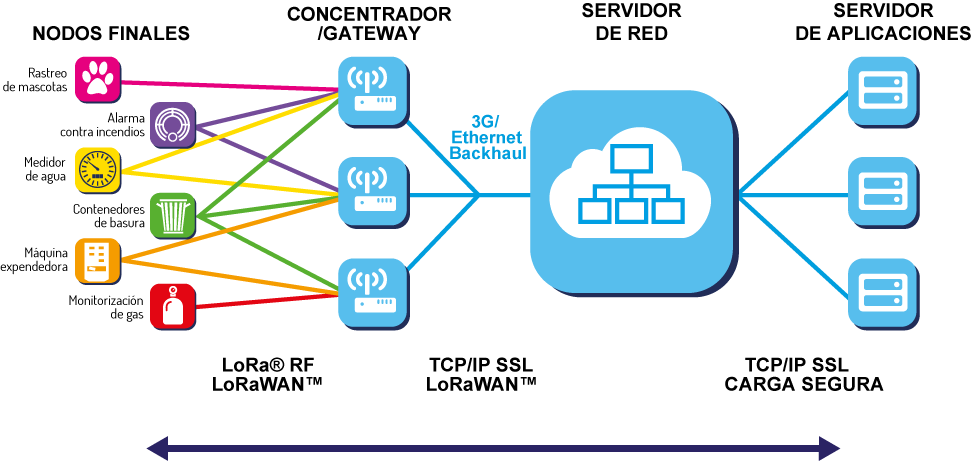
\includegraphics[width=16cm, height=8cm]{./Figuras/nodoLoraWan.png}
\caption{Arquitectura de red LoRaWAN}
\label{fig:arqLorawan}
\end{figure}

\vspace{25px}




\section{Identificación y análisis de los interesados}
\label{sec:interesados}

\begin{table}[ht]
%\caption{Identificación de los interesados}
%\label{tab:interesados}
\begin{tabularx}{\linewidth}{@{}|l|X|X|l|@{}}
\hline
\rowcolor[HTML]{C0C0C0} 
Rol           & Nombre y Apellido & Organización 	& Puesto 	\\ \hline
Cliente       & \clientename      &\empclientename	& -      	\\ \hline
Responsable   & \authorname       & FIUBA        	& Alumno 	\\ \hline
Orientador    & \supname	      & \pertesupname 	& Director	Trabajo final \\ \hline
Usuario final & Equipo de desarrollo de SW &INVAP S.E. & -        	\\ \hline
\end{tabularx}
\end{table}

\begin{itemize}
\item Cliente: es riguroso y exigente con la arquitecuta a desarrollar. Se recomienda hacer varias interconsultas para formalizar avances.
\item Orientador: Julieta Llanes, dispone de muy poco tiempo, usar las reuniones de manera eficiente.
\end{itemize}



\section{1. Propósito del proyecto}
\label{sec:proposito}

El propósito de este proyecto es solucionar los problemas hallados anteriormente en desarrollos similares y brindar al cliente un prototipo que permita futuros desarrollos IoT. Por otra parte, tiene como objetivo personal adquirir los conocimientos necesarios para elaborar proyectos de IoT por cuenta propia.

\section{2. Alcance del proyecto}
\label{sec:alcance}

El presente proyecto incluye: 

\begin{itemize}
\item Análisis y selección de RTOS.
\item Desarrollo de software en el nodo.
\item Desarrollo de visualizador de datos simple.
\item Armado de banco de pruebas.
\item Configuración de la red LoRaWAN.
\item Demostración funcional del nodo.
\end{itemize}

El presente proyecto no incluye: 
\begin{itemize}
\item Desarrollo de hardware.
\item Pruebas de campo.
\end{itemize}

\section{3. Supuestos del proyecto}
\label{sec:supuestos}

Para el desarrollo del presente proyecto se supone que:

\begin{itemize}
\item Tanto el hardware de desarrollo como el gateway serán provistos por el cliente.
\item El tiempo del desarrollo debe ser aproximadamente 600 hs.
\item Se contará con soporte técnico por parte de los directores.
\end{itemize}

\section{4. Requerimientos}
\label{sec:requerimientos}

\begin{enumerate}
\item Software del nodo
	\begin{enumerate}
	\item RN-001 Debe implementarse sobre un RTOS.
	\item RN-002 Debe permitir la administración de 1 a 4 sensores en simultáneo.
	\item RN-003 Debe enviar los datos recolectados de los sensores mediante un módem LoRa hacia un gateway utilizando un tiempo configurable para cada sensor.
	\item RN-004 Debe recibir comandos desde el gateway.
	\item RN-005 Debe poseer una arquitectura en capas e incorporar una HAL.
	\item RN-006 Debe poder ejecutarse en al menos 2 plataformas de HW diferentes.
	\item RN-007 Se debe utilizar control de versiones en GIT.
	\item RN-008 Se debe desarrollar un procedimiento de integración continua utilizando las herramientas provistas por la empresa cliente.
	\item RN-009 Debe poseer una arquitectura en capas.
	\item RN-010 Debe enviar información de estado.
	\end{enumerate}
\item Aplicación de usuario
	\begin{enumerate}
	\item RA-001 Debe recibir los mensajes provenientes del gateway.
	\item RA-002 Debe permitir el envío de comandos hacia el nodo.
	\item RA-003 Debe permitir la visualización de los mensajes recibidos.
	\end{enumerate}
\item Documentación
	\begin{enumerate}
	\item RD-001 La documentación debe ser generada con las herramientas de gestión de la empresa cliente.
	\end{enumerate}
\end{enumerate}

\section{Historias de usuarios (\textit{Product backlog})}
\label{sec:backlog}

Éstas historias fueron ponderadas según el volumen de trabajo y dificultad que implica satisfacer cada una de ellas utilizando la serie de Fibonacci.

\begin{itemize}
\item Como usuario quiero tener la posibilidad de utilizar diferentes sensores en simultáneo para poder medir diferentes propiedades físicas del entorno del nodo. (5)
\item Como analista de datos quiero disponer de una interfaz gráfica para visualizar la información proveniente de los sensores del nodo. (5)
\item Como analista de datos quiero visualizar información de los sensores conectados al nodo de manera remota para independizarme del lugar físico en el que se realizan las mediciones. (5)
\item Como analista de datos quiero configurar los tiempos de recolección y envío de datos de cada sensor, de ese modo se podrán obtener variaciones de las mediciones en diferentes períodos de tiempo. (3)
\item Como usuario encargado del mantenimiento del equipo quiero conocer el estado del nodo de manera remota para realizar un diagnóstico con facilidad. (1)
\item Como usuario encargado del mantenimiento del equipo quiero conocer el estado de la comunicación hacia el nodo de manera remota para realizar un diagnóstico con facilidad. (1)
\item Como miembro del equipo de desarrollo de software quiero cambiar fácilmente la plataforma de hardware para realizar una portabilidad hacia nuevos desarrollos. (8)
\end{itemize}

\section{5. Entregables principales del proyecto}
\label{sec:entregables}

\begin{itemize}
\item Documento de arquitectura de SW.
\item Instructivo de armado de banco de pruebas.
\item Documento de instalación de ambiente de desarrollo de SW.
\item Documento de análisis de RTOS.

\end{itemize}


\section{6. Desglose del trabajo en tareas}
\label{sec:wbs}

\begin{enumerate}
\item Introducción (134 hs)
	\begin{enumerate}
	\item Obtener información acerca de proyectos similares en la empresa y buscar referentes (12 hs)
	\item Gestionar envíos y compras de elementos necesarios (10 hs)
	\item Analizar documentación de las plataformas de HW a utilizar (15 hs)
	\item Obtener requerimientos iniciales (10 hs)
	\item Planificación del proyecto (15 hs)
	\item Armado de banco de pruebas (24 hs)
	\item Obtener información acerca de testing en sistemas embebidos (24 hs)
	\item Inducción a tecnologías LoRaWAN (24 hs)
	\end{enumerate}
\item Análisis y selección de RTOS (158 hs)
	\begin{enumerate}
	\item Estado del arte RTOS en IoT (24 hs)
	\item Análisis de arquitecturas multiplataforma en dispositivos IoT (40 hs)
	\item Instalación de SDK (24 hs)
	\item Diseño e implementación de pruebas de performance (40 hs)
	\item Ejecución de pruebas en 3 plataformas y análisis de resultados (30 hs)
	\end{enumerate}	
\item Software del nodo (120 hs)
	\begin{enumerate}
	\item Diseño (40 hs)
	\item Implementación (40 hs)
	\item Testing (40 hs)
	\end{enumerate}
\item Integración (78 hs)
	\begin{enumerate}
	\item Configuración gateway (8 hs)
	\item Diseño e implementación aplicación de usuario(40 hs)
	\item Testing y pruebas end to end (30 hs)
	\end{enumerate}
\item Gestión del proyecto (152 hs)
	\begin{enumerate}
	\item Reuniones de control y seguimiento del proyecto (40 hs)
	\item Elaboración de documentos para el cliente (40 hs)
	\item Elaboración de Memorias del proyecto (40 hs)
	\item Elaboración de presentación final del proyecto (32 hs)
	\end{enumerate}
\end{enumerate}

Cantidad total de horas: (642 hs)


\section{7. Diagrama de Activity On Node}
\label{sec:AoN}

En la Figura \ref{fig:AoN} se muestra el diagrama de \textit{Activity on Node} del proyecto. La unidad de tiempo está expresada en horas.
El camino crítico se representa en color naranja.
\begin{figure}[htpb]
\centering 
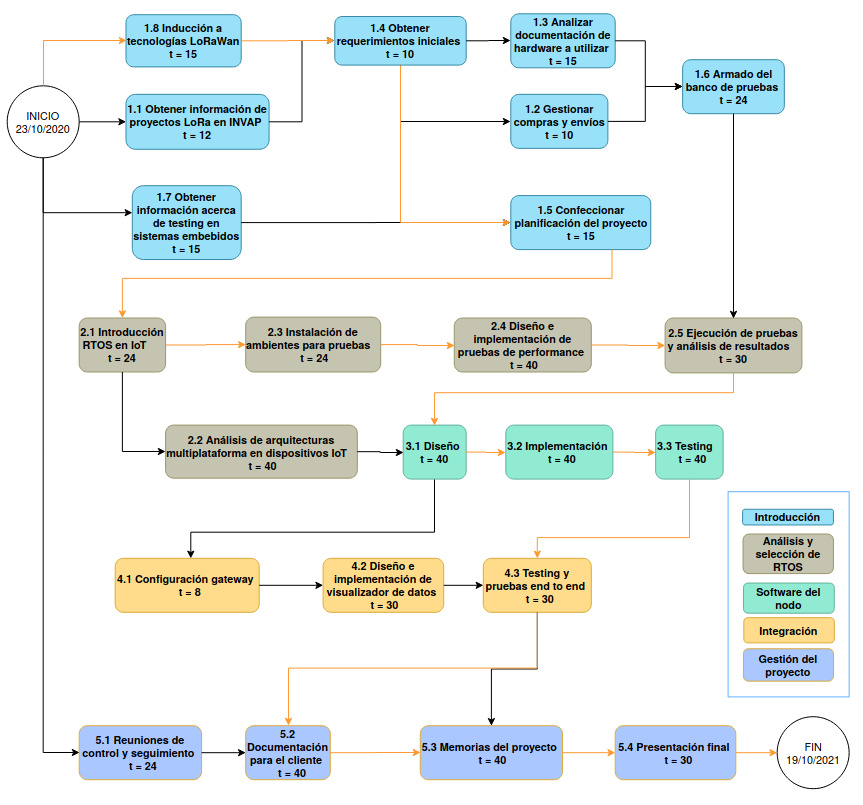
\includegraphics[width=16cm, height=15cm]{./Figuras/aon.png}
\caption{Diagrama \textit{Activity on Node}}
\label{fig:AoN}
\end{figure}



\section{8. Diagrama de Gantt}
\label{sec:gantt}

El diagrama de Gantt del proyecto se presenta en la Figura \ref{fig:Gantt}. En el mismo se pueden apreciar las fechas de inicio y finalización de cada tarea, así como también sus dependencias.

\begin{figure}[htpb]
\centering 
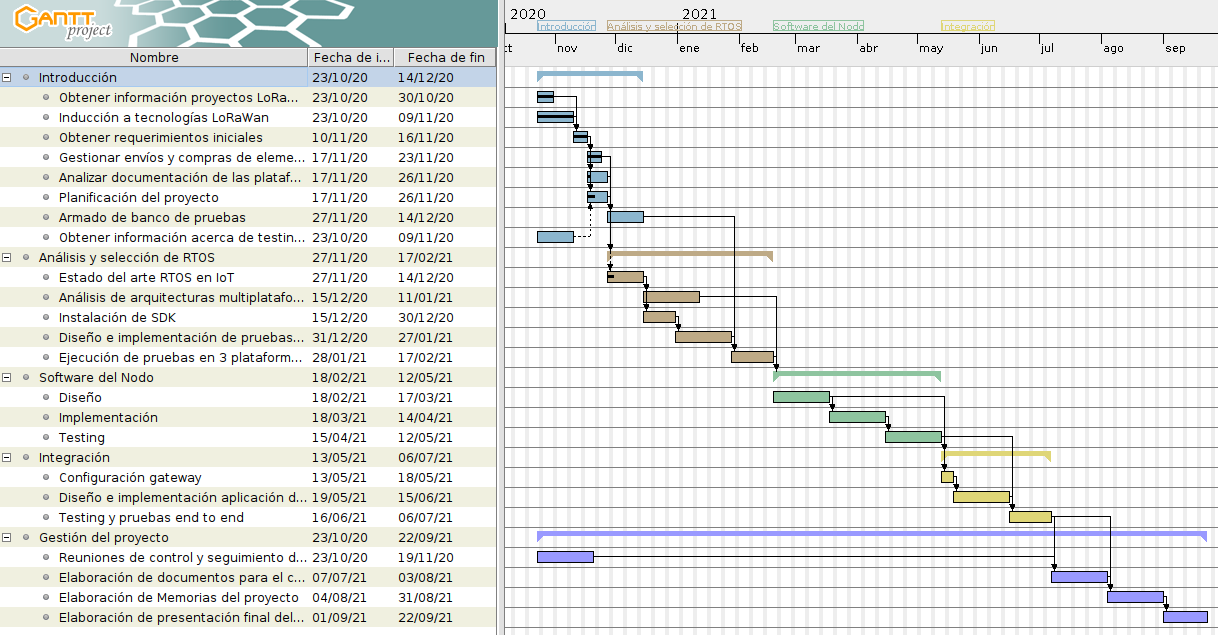
\includegraphics[width=16cm, height=10cm]{./Figuras/gantt.png}
\caption{Diagrama de \textit{Gantt}}
\label{fig:Gantt}
\end{figure}

\section{9. Matriz de uso de recursos de materiales}
\label{sec:recursos}

\begin{table}
\label{tab:recursos}
\centering
\begin{tabularx}{\linewidth}{@{}|c|X|X|X|X|c|@{}}
\hline
\cellcolor[HTML]{C0C0C0} & \cellcolor[HTML]{C0C0C0} & \multicolumn{3}{c|}{\cellcolor[HTML]{C0C0C0}Recursos requeridos (horas)} \\ \cline{3-5} 
\multirow{-2}{*}{\cellcolor[HTML]{C0C0C0}\begin{tabular}[c]{@{}c@{}}Código\\ WBS\end{tabular}} & \multirow{-2}{*}{\cellcolor[HTML]{C0C0C0}\begin{tabular}[c]{@{}c@{}}Nombre \\ tarea\end{tabular}} & PC & Banco de pruebas & Gateway \\ \hline
 1 &  Introducción & 110 & 24 &  \\ \hline
 2 &  Análisis y selección de RTOS & 158 & 70 &  \\ \hline
 3 &  Software nodo & 120 & 80 &  \\ \hline
 4 &  Integración & 70 & 30 & 8 \\ \hline
 5 &  Gestión del proyecto & 152 &  & \\ \hline

\end{tabularx}%
\end{table}


\section{10. Presupuesto detallado del proyecto}
\label{sec:presupuesto}

\begin{table}[htpb]
\centering
\begin{tabularx}{\linewidth}{@{}|X|c|r|r|@{}}
\hline
\rowcolor[HTML]{C0C0C0} 
\multicolumn{4}{|c|}{\cellcolor[HTML]{C0C0C0}COSTOS DIRECTOS} \\ \hline
\rowcolor[HTML]{C0C0C0} 
Descripción &
  \multicolumn{1}{c|}{\cellcolor[HTML]{C0C0C0}Cantidad} &
  \multicolumn{1}{c|}{\cellcolor[HTML]{C0C0C0}Valor unitario} &
  \multicolumn{1}{c|}{\cellcolor[HTML]{C0C0C0}Valor total} \\ \hline
 Horas de ingeniería & 
  \multicolumn{1}{c|}{642} & 
  \multicolumn{1}{c|}{500} & 
  \multicolumn{1}{c|}{321000} \\ \hline

\multicolumn{3}{|c|}{SUBTOTAL} &
  \multicolumn{1}{c|}{321000} \\ \hline
\rowcolor[HTML]{C0C0C0} 
\multicolumn{4}{|c|}{\cellcolor[HTML]{C0C0C0}COSTOS INDIRECTOS} \\ \hline
\rowcolor[HTML]{C0C0C0} 
Descripción &
  \multicolumn{1}{c|}{\cellcolor[HTML]{C0C0C0}Cantidad} &
  \multicolumn{1}{c|}{\cellcolor[HTML]{C0C0C0}Valor unitario} &
  \multicolumn{1}{c|}{\cellcolor[HTML]{C0C0C0}Valor total} \\ \hline
\multicolumn{1}{|l|}{30 \% costos directos} &
\multicolumn{1}{c|}{642} & 
  \multicolumn{1}{c|}{150} & 
  \multicolumn{1}{c|}{96300} \\ \hline
  
\multicolumn{3}{|c|}{SUBTOTAL} &
  \multicolumn{1}{c|}{96300} \\ \hline
\rowcolor[HTML]{C0C0C0}
\multicolumn{3}{|c|}{TOTAL} & 417300
   \\ \hline
\end{tabularx}%
\end{table}


\section{11. Matriz de asignación de responsabilidades}
\label{sec:responsabilidades}

\begin{table}[htpb]
\centering
\resizebox{\textwidth}{!}{%
\begin{tabular}{|c|c|c|c|c|c|}
\hline
\rowcolor[HTML]{C0C0C0} 
\cellcolor[HTML]{C0C0C0} &
  \cellcolor[HTML]{C0C0C0} &
  \multicolumn{3}{c|}{\cellcolor[HTML]{C0C0C0}Listar todos los nombres y roles del proyecto} \\ \cline{3-5} 
\rowcolor[HTML]{C0C0C0} 
\cellcolor[HTML]{C0C0C0} &
  \cellcolor[HTML]{C0C0C0} &
  Responsable &
  Orientador &
  Cliente \\ \cline{3-5} 
\rowcolor[HTML]{C0C0C0} 
\multirow{-3}{*}{\cellcolor[HTML]{C0C0C0}\begin{tabular}[c]{@{}c@{}}Código\\ WBS\end{tabular}} &
  \multirow{-3}{*}{\cellcolor[HTML]{C0C0C0}Nombre de la tarea} &
  \authorname &
  \supname &
  \clientename \\ \hline
 1& Introducción & P & A & C \\ \hline
 2& Análisis RTOS & P & S & A \\ \hline
 3& Software Nodo & P & S & A \\ \hline
 4& Integración & P & I & A\\ \hline
 5& Gestión del proyecto & P & A & A \\ \hline
\end{tabular}%
}
\end{table}

{\footnotesize
Referencias:
\begin{itemize}
	\item P = Responsabilidad Primaria
	\item S = Responsabilidad Secundaria
	\item A = Aprobación
	\item I = Informado
	\item C = Consultado
\end{itemize}
} %footnotesize

\section{12. Gestión de riesgos}
\label{sec:riesgos}

a) Identificación de los riesgos (al menos cinco) y estimación de sus consecuencias:
 
Riesgo 1: No disponer del tiempo suficiente para llevar a cabo el proyecto
\begin{itemize}
\item Severidad (8): Implica que la fecha de entrega será posterior a la estimada.
\item Probabilidad de ocurrencia (7): El responsable del proyecto posee una jornada laboral de 9 horas y se encuentra cursando la CESE, ello implica 9 horas de cursada semanales y otras 6 horas semanales para dedicarle a los trabajos solicitados por parte de la cátedra. 
\end{itemize}   

Riesgo 2: Mala planificación del proyecto
\begin{itemize}
\item Severidad (8): Implica que la fecha de entrega será posterior a la estimada.
\item Ocurrencia (8): Generalmente la falta de experiencia en la gestión de proyectos y la subestimación de tiempos para realizar las tareas debido al conocimiento parcial con el que se cuenta al realizar la planificación hacen que este riesgo sea altamente probable.
\end{itemize}

Riesgo 3: Poca interacción con el cliente
\begin{itemize}
\item Severidad (6): Implica que el producto a realizar pueda ser diferente a lo esperado por el cliente, los tiempos se pueden extender debido a modificaciones en el alcance del proyecto. 
\item Ocurrencia (8): El cliente ha demostrado bajo nivel de disponibilidad, hay una demora considerable al intentar establecer una comunicación con él. 
\end{itemize}

Riesgo 4: Viajes en fechas imprevistas
\begin{itemize}
\item Severidad (3): Implica retrasos en los avances del proyecto debido a que durante ese tiempo no se contará con el setup de desarrollo.
\item Ocurrencia (4): El responsable del proyecto tiene un viaje planificado que se ha reprogramado en diversas ocasiones debido los problemas actuales a nivel global (COVID-19)
\end{itemize}

Riesgo 5: Retrasos para conseguir hardware
\begin{itemize}
\item Severidad (2): Implica retrasos en los avances del proyecto debido a que durante ese tiempo no se contará con el setup de desarrollo.
\item Ocurrencia (8): Los componentes necesarios para el armado del banco de pruebas se encuentran en la ciudad de Córdoba. Es altamente probable que se demoren los envíos.
\end{itemize}

Riesgo 6: Aislamiento COVID-19
\begin{itemize}
\item Severidad (5): Implica retrasos en los avances del proyecto debido a que durante ese tiempo no se contará con el setup de desarrollo.
\item Ocurrencia (7): Los rebrotes actuales en diferentes lugares del mundo, dan a entender que el año 2021 podríamos tener cuarentena estricta nuevamente.
\end{itemize}

b) Tabla de gestión de riesgos:      (El RPN se calcula como RPN=SxO)

\begin{table}[htpb]
\centering
\begin{tabularx}{\linewidth}{@{}|X|c|c|c|c|c|c|@{}}
\hline
\rowcolor[HTML]{C0C0C0} 
Riesgo & S & O & RPN & S* & O* & RPN* \\ \hline
   No disponer del tiempo suficiente para llevar a cabo el proyecto    &  8 &  7 &  56   &  8  &  3  &  24    \\ \hline
   Mala planificación del proyecto    &  8 &  8 &  64   &  6  &  3  &  18    \\ \hline
   Poca interacción con el cliente    &  6 &  8 &  48   &  3  &  8  &  24    \\ \hline
   Viajes en fechas imprevistas    &  3 &  4 &  12   &    &    &      \\ \hline
   Retrasos para conseguir hardware    &  2 &  8 &  16   &    &    &      \\ \hline
   Aislamiento COVID-19    &  5 &  7 &  35   &  4  &  7  &  28    \\ \hline
\end{tabularx}%
\end{table}

Criterio adoptado: 
Se tomarán medidas de mitigación en los riesgos cuyos números de RPN sean mayores a 30

Nota: los valores marcados con (*) en la tabla corresponden luego de haber aplicado la mitigación.

c) Plan de mitigación de los riesgos que originalmente excedían el RPN máximo establecido:
 
\textbf{Riesgo 1: } El plan de mitigación consiste en gestionar una cantidad de horas dentro de la jornada de trabajo. El proyecto se realizará para la empresa en la que el principal responsable de llevarlo a cabo trabaja actualmente.
  
  - Severidad (8): La severidad se mantiene.
  
  - Probabilidad de ocurrencia (3): Disminuye la probabilidad de ocurrencia debido a que se dipondrá de una cantidad de horas mayor.

\textbf{Riesgo 2: } El plan de mitigación consiste en involucrar a los directores en el armado de la planificación.
  
  - Severidad (8): La severidad se mantiene.
  
  - Probabilidad de ocurrencia (3): Al contar con la colaboración de gente experimentada en gestión de proyectos, la probabilidad de ocurrencia disminuye.

 
\textbf{Riesgo 3: } El plan de mitigación consiste en consensuar con el cliente un alcance claro del proyecto, se requiere un feedback de la especificación de requeriemientos.
  
  - Severidad (3): Al tener el alcance claro, la severidad de tener poca comunicación es menor.
  
  - Probabilidad de ocurrencia (8): La probabilidad de ocurrencia se mantiene.

\textbf{Riesgo 6: } El plan de mitigación consiste en utilizar la mayor cantidad de recursos posibles para trabajar de manera remota.
  
  - Severidad (4): Al poder trabajar de manera remota, la severidad de tener poca comunicación es menor, el valor es 4 porque algunas tareas no se van a poder realizar de manera remota.
  
  - Probabilidad de ocurrencia (7): La probabilidad de ocurrencia se mantiene.

\section{13. Gestión de la calidad}
\label{sec:calidad}

\begin{consigna}{red}
Para cada uno de los requerimientos del proyecto indique:
\begin{itemize} 
\item Req \#1: copiar acá el requerimiento.

Verificación y validación:

\begin{itemize}
\item Verificación para confirmar si se cumplió con lo requerido antes de mostrar el sistema al cliente. Detallar 
\item Validación con el cliente para confirmar que está de acuerdo en que se cumplió con lo requerido. Detallar  
\end{itemize}

\end{itemize}

Tener en cuenta que en este contexto se pueden mencionar simulaciones, cálculos, revisión de hojas de datos, consulta con expertos, mediciones, etc.

\end{consigna}

\section{14. Comunicación del proyecto}
\label{sec:comunicaciones}

El plan de comunicación del proyecto es el siguiente:

\begin{table}[htpb]
\centering
\begin{tabularx}{\linewidth}{@{}|X|C{2.4cm}|C{3cm}|C{1.8cm}|C{2cm}|C{2.1cm}|@{}}
\hline
\rowcolor[HTML]{C0C0C0} 
\multicolumn{6}{|c|}{\cellcolor[HTML]{C0C0C0}PLAN DE COMUNICACIÓN DEL PROYECTO}           \\ \hline
\rowcolor[HTML]{C0C0C0} 
¿Qué comunicar? & Audiencia & Propósito & Frecuencia & Método de comunicac. & Responsable \\ \hline
                &           &           &            &                      &             \\ \hline
                &           &           &            &                      &             \\ \hline
                &           &           &            &                      &             \\ \hline
                &           &           &            &                      &             \\ \hline
                &           &           &            &                      &             \\ \hline
\end{tabularx}
\end{table}

\section{15. Gestión de compras}
\label{sec:compras}

Éste proyecto no requiere la compra de componentes dado que se los materiales ya están disponibles en la empresa cliente.

\section{16. Seguimiento y control}
\label{sec:seguimiento}

\begin{consigna}{red}
Para cada tarea del proyecto establecer la frecuencia y los indicadores con los se seguirá su avance y quién será el responsable de hacer dicho seguimiento y a quién debe comunicarse la situación (en concordancia con el Plan de Comunicación del proyecto).

El indicador de avance tiene que ser algo medible, mejor incluso si se puede medir en \% de avance. Por ejemplo,se pueden indicar en esta columna cosas como ``cantidad de conexiones ruteadeas'' o ``cantidad de funciones implementadas'', pero no algo genérico y ambiguo como ``\%'', porque el lector no sabe porcentaje de qué cosa.

\end{consigna}

\begin{longtable}{|m{1cm}|m{3.5cm}|m{2.2cm}|m{2cm}|m{3cm}|m{1.5cm}|}
\hline
\rowcolor[HTML]{C0C0C0} 
\multicolumn{6}{|c|}{\cellcolor[HTML]{C0C0C0}SEGUIMIENTO DE AVANCE}                                                                       \\ \hline
\rowcolor[HTML]{C0C0C0} 
Tarea del WBS 			& Indicador de avance & Frecuencia de reporte & Resp. de seguimiento & Persona a ser informada & Método de comunic. \\ \hline
\endfirsthead

\hline
\rowcolor[HTML]{C0C0C0} 
\multicolumn{6}{c}{\cellcolor[HTML]{C0C0C0}SEGUIMIENTO DE AVANCE}                                                                       \\ \hline
\rowcolor[HTML]{C0C0C0} 
Tarea del WBS 			& Indicador de avance & Frecuencia de reporte & Resp. de seguimiento & Persona a ser informada & Método de comunic. \\ \hline
\endhead

\multicolumn{6}{c}{Continúa}
\endfoot

\endlastfoot

1.1	& Fecha de inicio  & Única vez al comienzo & \authorname & \clientename, \supname & email \\ \hline
2.1	& Avance de las subtareas  & Mensual mientras dure la tarea & \authorname & \clientename, \supname & email \\ \hline

\end{longtable}

\begin{table}[!htpb]
\centering
%\begin{tabularx}{\linewidth}{@{}|X|X|X|X|X|X|@{}}
\begin{tabularx}{\linewidth}{@{}|X|C{2.5cm}|C{3cm}|C{2cm}|C{2cm}|C{2.5cm}|@{}}
\hline
\rowcolor[HTML]{C0C0C0} 
\multicolumn{6}{|c|}{\cellcolor[HTML]{C0C0C0}SEGUIMIENTO DE AVANCE}                                                                       \\ \hline
\rowcolor[HTML]{C0C0C0} 
Tarea del WBS & Indicador de avance & Frecuencia de reporte & Resp. de seguimiento & Persona a ser informada & Método de comunic. \\ \hline
 &  &  &  &  &  \\ \hline
 &  &  &  &  &  \\ \hline
 &  &  &  &  &  \\ \hline
 &  &  &  &  &  \\ \hline
 &  &  &  &  &  \\ \hline
\end{tabularx}%
%}
\end{table}

\section{17. Procesos de cierre}    
\label{sec:cierre}

\begin{consigna}{red}
Establecer las pautas de trabajo para realizar una reunión final de evaluación del proyecto, tal que contemple las siguientes actividades:

\begin{itemize}
\item Pautas de trabajo que se seguirán para analizar si se respetó el Plan de Proyecto original:
 - Indicar quién se ocupará de hacer esto y cuál será el procedimiento a aplicar. 
\item Identificación de las técnicas y procedimientos útiles e inútiles que se utilizaron, y los problemas que surgieron y cómo se solucionaron:
 - Indicar quién se ocupará de hacer esto y cuál será el procedimiento para dejar registro.
\item Indicar quién organizará el acto de agradecimiento a todos los interesados, y en especial al equipo de trabajo y colaboradores:
  - Indicar esto y quién financiará los gastos correspondientes.
\end{itemize}

\end{consigna}


\end{document}
